\def\year{2018}\relax
%File: formatting-instruction.tex
\documentclass[letterpaper]{article} %DO NOT CHANGE THIS
\usepackage{aaai18}  %Required
\usepackage{times}  %Required
\usepackage{helvet}  %Required
\usepackage{courier}  %Required
\usepackage{url}  %Required
\usepackage{graphicx}  %Required
%\usepackage{dblfloatfix}
\usepackage{stfloats}
\frenchspacing  %Required
\setlength{\pdfpagewidth}{8.5in}  %Required
\setlength{\pdfpageheight}{11in}  %Required
%PDF Info Is Required:
  \pdfinfo{
/Title (2018 Formatting Instructions for Authors Using LaTeX)
/Author (AAAI Press Staff)}
%\setcounter{secnumdepth}{2}  

%\usepackage{etoolbox}
%\newcommand{\zerodisplayskips}{%
%	\setlength{\abovedisplayskip}{0pt}%
%	\setlength{\belowdisplayskip}{0pt}%
%	\setlength{\abovedisplayshortskip}{0pt}%
%	\setlength{\belowdisplayshortskip}{0pt}}
%\appto{\normalsize}{\zerodisplayskips}
%\appto{\small}{\zerodisplayskips}
%\appto{\footnotesize}{\zerodisplayskips}
%\usepackage{enumitem}
%\setlist{nosep}

\usepackage{CJKutf8}
\usepackage{amsmath,amsfonts,amsthm}
\usepackage{color}
\usepackage{array}
\usepackage{epsfig}
\usepackage{caption}
\usepackage{subcaption}
\usepackage{array}
\usepackage{ragged2e}
\usepackage{pbox}
\usepackage{enumitem}
\setenumerate[1]{itemsep=0pt,partopsep=0pt,parsep=\parskip,topsep=5pt}
\setitemize[1]{itemsep=0pt,partopsep=0pt,parsep=\parskip,topsep=5pt}
\setdescription{itemsep=0pt,partopsep=0pt,parsep=\parskip,topsep=5pt}

\usepackage[ruled,vlined,boxed,linesnumbered]{algorithm2e}
\SetAlFnt{\small}
\SetAlCapFnt{\small}
\SetAlCapNameFnt{\small}
\usepackage{float}
\restylefloat{table}
\newcolumntype{P}[1]{>{\RaggedRight\hspace{0pt}}p{#1}}
\newcolumntype{L}[1]{>{\raggedright\let\newline\\\arraybackslash\hspace{0pt}}m{#1}}
\newcolumntype{C}[1]{>{\centering\let\newline\\\arraybackslash\hspace{0pt}}m{#1}}
\newcolumntype{R}[1]{>{\raggedleft\let\newline\\\arraybackslash\hspace{0pt}}m{#1}}


\newcommand{\secref}[1]{Section \ref{#1}}
\newcommand{\figref}[1]{Figure \ref{#1}}
\newcommand{\eqnref}[1]{Eq. (\ref{#1})}
\newcommand{\tabref}[1]{Table \ref{#1}}
\newcommand{\exref}[1]{Example \ref{#1}}
\newcommand{\algref}[1]{Algorithm \ref{#1}}
\newcommand{\socvec}{SocVec}
\newcommand{\argmin}{\operatornamewithlimits{argmin}}
\newcommand{\argmax}{\operatornamewithlimits{argmax}}
\newtheorem{example}{Example}
\newtheorem{lemma}{Lemma}
\newtheorem{definition}{Definition}
\newcommand{\cut}[1]{}

\newcommand{\li}{\uline{\hspace{0.5em}}}
\newcommand{\BL}[1]{\textcolor{blue}{Bill: #1}}
\newcommand{\HY}[1]{\textcolor{red}{Hanyuan: #1}}
\newcommand{\KZ}[1]{\textcolor{green}{Kenny: #1}}
\newcommand{\SH}[1]{\textcolor{green}{Seung: #1}}
\newcommand{\FX}[1]{\textcolor{blue}{Frank: #1}}

\begin{document}
% The file aaai.sty is the style file for AAAI Press 
% proceedings, working notes, and technical reports.
%
\title{Understanding Slang Terms across Languages}
\author{
		Bill Y. Lin\thanks{Phone: +86 13120889217; URL: https://yuchenlin.github.io},
		Frank F. Xu and
		Kenny Q. Zhu
		\\[0.5ex]
		\url{{yuchenlin, frankxu}@sjtu.edu.cn, kzhu@cs.sjtu.edu.cn}\\[0.5ex]
		Department of Computer Science and Engineering\\[0.5ex]
		Shanghai Jiao Tong University\\[0.5ex]
		800 Dongchuan Road, Shanghai, China 200240
}
\maketitle
\begin{abstract}
Understanding slang terms across languages is an important challenge in bilingual text understanding, machine translation and cross-cultural communication.
In this paper, we propose a novel task to  find terms in one language that can help explain given slang terms in another language. 
We also release the very first benchmark dataset as well as some baseline methods regarding this task.
%This paper presents a novel framework for obtaining bilingual
%word representations from social media by leveraging ``social vocabularies''. 
%Such representations can act as a building block for cross-lingual and cross-cultural studies in computational social science.
%We evaluate our framework on two tasks: 
%1) detection of cross-cultural differences of named entities in social media
%and 
%2) 
%We also release two new datasets for these tasks.
Based on social media corpora and existing work on cross-lingual word representation, we propose a straightforward but effective approach (\textit{\socvec}). 
Experimental results show that our approach outperforms  sophisticated baseline methods by 
substantial margins.
\end{abstract}
\begin{CJK}{UTF8}{gkai}
	\section{Introduction}
\label{sec:intro}
Slang terms are widely used in social media and novel slang terms emerge all the time, but understanding such slang terms across languages can be a very challenging task.
Consider the following question:
 {\em What are the English terms that can help us understand the meaning of the Chinese slang term``浮云''? \footnote{{\scriptsize ``浮云'' is a Chinese slang term, which literally means ``floating clouds''. However,  it almost always means something as ephemeral and unimportant as ``passing clouds'', both on the Internet and in everyday life.}}} 
We find that both existing dictionaries and state-of-the-art machine translators often just translate such slang terms to their literal meanings, 
even under a clear context where slang meanings are much more appropriate.  

Given a slang term in one language, our research problem is to find terms in another language which can help people understand its meaning.
We believe this research area not only can assist people to communicate better in cross-cultural situations but also improves the performance of existing machine translation systems.  
Attacking this research problem, we make the following contributions in this paper:
\begin{enumerate}
	\itemsep0em 
	\item To the best of our knowledge, we are the first to propose a task about understanding slang cross-lingually. 
	We also provide a benchmark dataset for evaluation which can benefit  further research in this area. 
	
	\item We propose a straightforward but effective approach to build bilingual word representations (\textit{\socvec}) from social media. 
	With \textit{\socvec}, we can simply compute cross-lingual word similarities to find target terms. 
	\item Qualitative and quantitative evaluation  show that our proposed approach outperforms the baseline methods.
\end{enumerate}
%\vspace{-10pt}
\section{Dataset Building and Task Description}
%\vspace{-10pt}
We first introduce how we build our dataset for the proposed task.\footnote{{\scriptsize Due to the salient cross-cultural differences between the east and the west, we choose English and Chinese as the example language pair in this paper.}} 
We use an online Chinese slang glossary\footnote{\tiny{\url{https://www.chinasmack.com/glossary}}} consisting of  200 popular slang terms with English explanations to construct the ground truth target English terms by extracting most related words.  
%For each Chinese slang term, we extract the ground truth target English terms from its explanation in the glossary, which can help people understand their slang meanings.  
For example, we extract the most relevant words (boldfaced) in the glossary entry of the Chinese slang term ``二百五'' as follows:
\begin{description}
%	\vspace{-10pt}
	\item[二百五]: A \textbf{\textit{foolish}} person who is lacking in sense but still \textbf{\textit{stubborn}}, \textbf{\textit{rude}}, and \textbf{\textit{impetuous}}.
\end{description}
Similarly for English slang terms, we resort to a slang word list from OnlineSlangDictionary\footnote{\tiny{\url{http://onlineslangdictionary.com/word-list/}}} with translated explanations and then down-sample the list to 200 terms as well.  
%Similarly, for each English slang term of interest, we extract the important words from its explanation and then utilize their translations as the final ground truth.
%
%Different methods should produce a list of translation terms 
%as similar as possible to the ground truth target terms.
%Finally, for each English or Chinese slang term, we have a set of target Chinese or English terms which are considered to be helpful for understanding slang across languages.

Given any slang term in a \textit{source} language in this dataset, our proposed task is to find a set of words in another \textit{target} language that should be close to the ground truth word set. 
\vspace{-5pt}
\section{Baseline Methods}
We propose two types of baseline methods for this task. 
The first type is based on well-known {\em on-line translators}, 
namely Google, 
Bing and Baidu.  
%With our test set's slang as input, we retrieve the output of translation. 
A specific baseline method for Chinese slang is from CC-CEDICT\footnote{{\scriptsize An on-line public-domain Chinese-English dictionary, which is well updated with popular slang terms. \url{https://cc-cedict.org/wiki/}}} (CC).
%Considering situations that many slang terms have literal meaning, it is unfair to retrieve target terms from such on-line translators by simply inputing slang terms without slang contexts. 
%We use example sentences with slang terms from some websites (mainly from Urban 
%Dictionary\footnote{\scriptsize{\url{http://www.urbandictionary.com/}}}) 
%as input for such translators, so that they are expected to have a great chance of knowing this is
%a slang use. 
%\footnote{Nevertheless, we noticed
%	that the on-line translators often ignore the slang contexts and still produce
%	literal translations.}
%The following example shows how we obtain the target translation terms 
%for the slang word ``fruitcake'' (an insane person) from Google Translator:

%\noindent
%\textit{Input Sentence:}
%{\textit{Oh man, you don't want to date that girl. She's always drunk and yelling. She is a total \underline{fruitcake}.}}\footnote{{\url{http://www.englishbaby.com/lessons/4349/slang/fruitcake}}}\\ 
%\textit{Google Translation:}
%{\small哦, 男人, 你不想约会那个女孩。她总是喝醉了, 大喊大叫。她是一个\underline{水果蛋糕}。}

The second type of baseline methods are ranking based. 
We score each of the possible term in the target language and consider the top five as the target 
terms. 
%Given a source term to be translated, several such {\em ranking-based 
%	baseline methods} are as follows.
Existing \textit{cross-lingual word representation} models can be applied to compute the semantic similarities of terms across languages.
Thus, we score all candidate target terms by computing cosine similarities in their constructed bilingual vector spaces with different models: Linear Transform (LT)~\cite{Mikolov:2013tp}, MultiCCA, MultiCluster~\cite{ammar2016massively} and Duong~\cite{DBLP:conf/emnlp/DuongKMBC16} methods. 
A more sophisticated baseline method, TransBL, first translates each candidate target term back into the source language with a bilingual dictionary. Then, we calculate the average cosine similarities between the source term and the translated terms in monolingual word vector space as the scores to rank. 
\vspace{-10pt}
\section{\socvec ~Model}
\begin{figure}[]
	\centering
	\caption{Workflow for computing the cross-cultural similarity between 
		an English word \textit{W} and a Chinese word \textit{U}.}
	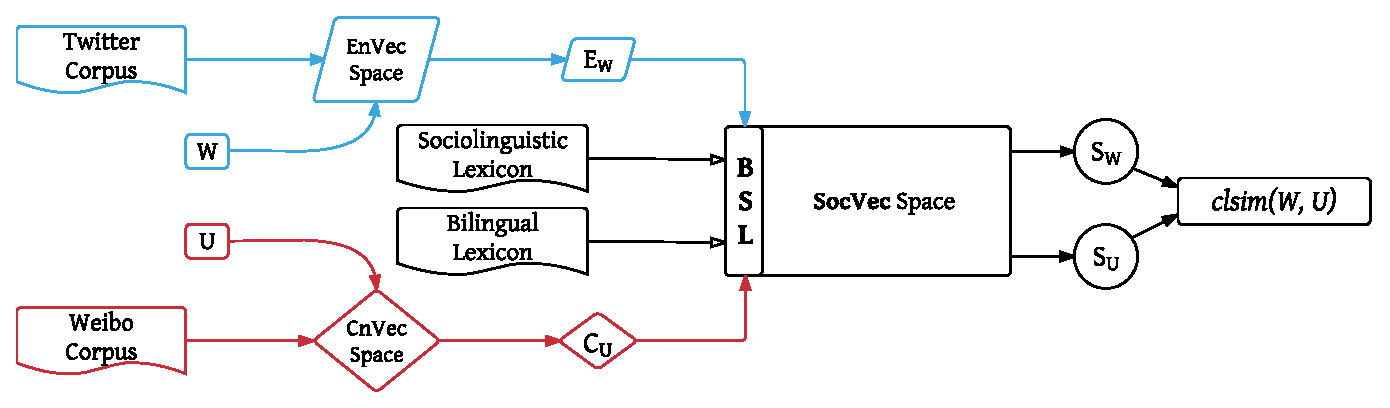
\epsfig{file=figures/overview.pdf, width=0.5\columnwidth}
	
	\label{fig:overview}
	\vspace{-10pt}
\end{figure}
In this paper, we propose a novel approach to project 
two heterogeneous monolingual word vector spaces into 
one bilingual word vector space, known as 
social vector space (\textit{\socvec}), 
by constructing a bilingual social lexicon (BSL) consisting of bilingual mappings of selected \textit{social word}s
that reflect opinion, sentiment, cognition and many other psychological 
processes. 
These words, we believe, are central to capturing cultural semantics.
%using only a bilingual lexicon (for common words), two monolingual socio-linguistic vocabularies and a comparable corpus\footnote{A comparable corpus is a pair of corpora in two different languages, which come from the same domain.} from microblogs, all of which are easily available.

Each dimension of our \textit{\socvec}~then represents a \textit{socio-linguistic} feature 
derived from mono-lingual semantic similarities between an input term and 
each corresponding entry in the BSL. 
Consequently, a term $W$ in language $L_1$ and a term $U$ in 
language $L_2$ can each be respectively projected 
into a bilingual word vector in the \textit{\socvec} while maintaining
their social features. Thus, cross-cultural similarities can be computed directly with vectors from \textit{SocVec}. 

\figref{fig:overview} shows the overall workflow of our approach to construct the \textit{SocVec} and compute cross-lingual similarity between $W$ and $U$, denoted as $\text{clsim}(W,U)$. 
\footnote{{\scriptsize Notations are as follows: CnVec = Chinese word vector space, EnVec = English word vector space, CSV = Chinese social word vocab, ESV = English social word vocab, BL = Bilingual Lexicon, BSL = Bilingual Social Lexicon.
Finally, $\mathbf{E_x}$, $\mathbf{C_x}$ and $\mathbf{S_x}$ are the word vectors of word $x$ (either $U$ or $W$) in EnVec space, CnVec space and SocVec space respectively.}} 
With such cross-lingual similarities, we can easily compute the score of each candidate target terms like other ranking-based baseline methods explored above.       
%Thanks to the large size of our social word vocabulary and the developing process,(around 3k-5k)  
%Note that \textit{ScoVec} is an encoding for words across languages, where each dimension has 
%clear meaning.
\section{Evaluation}
We first show two 
examples of translations of different methods for qualitative evaluation:
% && Water army& Navy& Navy & propaganda, complicit, fraudulent
\begin{description}
	%	\vspace{-10pt}
	\item[1) 水军] This slang term literally means ``water army'', but its slang meaning is the people paid to slander competitors on the Internet and to help shape public opinion. The results of Google, Bing and Baidu translators are \textbf{``\textit{Water} \textit{Navy}''}, which is the literal meaning of this slang term. However, our \textit{\socvec}  can produce words such as \textbf{{``\textit{propaganda}'', ``\textit{complicit}'', ``\textit{fraudulent}''}}, reflecting its real slang meanings.
	
	\item[2) fruitcake] This slang term means a crazy person, or someone who is completely insane. 
	We found that all online translators treat it as ``\textit{\textbf{fruit cake}}'', even given a context like ``\textit{She’s always drunk and yelling, and she is a total fruitcake.}''\footnote{{\tiny \url{ http://www.englishbaby.com/lessons/4349/
slang/fruitcake}}}. 
	In contrast, our method can capture the slang meaning and produce words like \textbf{``厌烦''{\textit{(annoying)}}, ``疯狂''\textit{(crazy)} } and \textbf{ ``怪诞''\textit{(bizarre)}.}
\end{description} 
% 
%Our results are highly correlated with these explanations and capture their core semantics, whereas most online translators just offer literal translation of such slang terms, even with the ample slang contexts.

To quantitatively evaluate different methods, we need to measure similarities between the produced target term sets and the ground truth word sets.
Exact-matching based similarity is too strict to capture valuable relatedness between two word sets.  
We argue that the\textit{ Average Cosine Similarity} (ACS) between two sets of word vectors is a better metric to evaluate the similarity between two word sets:
\begin{align*}
\vspace{-3pt}
ACS (A,B)=
{\frac{1}{|A||B|}}{\sum_{i=1}^{|A|}{\sum_{j=1}^{|B|}} \frac{\mathbf{A_i }\cdot \mathbf{B_j}}{\|\mathbf{A_i }\|\|\mathbf{B_j }\|}}
\vspace{-2pt}
\end{align*} 
where $A$ and $B$ are the two word sets; $\mathbf{A_i}$ and $\mathbf{B_j}$ are the two word vectors of the $i^{th}$ word in $A$ and $j^{th}$ in $B$ respectively\footnote{{\scriptsize The word vectors used in ACS computation is a third-party pre-trained 
		embedding and thus ACS computation is fair over different methods.}}. 
\tabref{tab:bleis_acs} shows the quantitative evaluation results. 
\begin{table}[] 
	\caption{ACS Sum Results of Slang Translation 	\vspace{-10pt}}
	\small
	\centering
	\begin{subtable}[h]{0.9\columnwidth}
		\centering
		\begin{tabular}{|ccccc|}
			\hline
			Google&  Bing& Baidu & CC & LT   \\ 
			18.24 &  16.38&  17.11 & 17.38 & 9.14 \\ \hline
			TransBL& MultiCCA & MultiCluster & Duong   & \textbf{\socvec} \\ 
			18.13 &  17.29 & 17.47&  20.92& \textbf{23.01}\\ \hline  
		\end{tabular}
		\subcaption{Chinese Slang to English}
	\end{subtable}
	\begin{subtable}[h]{0.9\columnwidth}
		\centering
		\begin{tabular}{|ccccc|}
			\hline
			Google&  Bing& Baidu &  LT   & TransBL\\ 
			6.40  &   15.96 &  15.44  & 7.32 & 11.43\\    \hline
			MultiCCA & MultiCluster & Duong   & \textbf{\socvec} & \\ 
			15.29 & 14.97&  15.13& \textbf{17.31} & \\ \hline  
		\end{tabular}
		\subcaption{English Slang to Chinese}
	\end{subtable}
	
	\label{tab:bleis_acs}
\end{table}

\vspace{-5pt}
\section{Conclusion and Future Work} 
We propose a novel task about understanding slang across languages with a benchmark data set. Also, experiments show that our proposed \socvec~ based method is more effective than other strong baseline methods. 
Future directions include further development of larger datasets for more languages and then proposing supervised methods.

 
%	\section{Approach}
\label{sec:socvec}
We first discuss the intuition behind our model informally, then give the overall workflow of our approach, and finally present the details of the~\textit{\socvec}~framework. 

\subsection{Problem Statement and the Intuition}
Assuming the language $L_1$ is English and $L_2$ is Chinese,\footnote{Since the cross-cultural differences between eastern and western cultures are salient, 
this paper mainly considers English and Chinese as the target languages. 
Nevertheless, the techniques developed here are language independent and 
thus can be used for any two natural languages so long as 
we have a bilingual lexicon for the pair and a social-linguistic lexicon 
for one of the languages.} the problem we want to solve is, given 
an English term $W$ and a Chinese term $U$, compute a cross-lingual 
similarity score, $clsim(W, U)$, representing the cross-cultural 
similarity between $W$ and $U$. 

Although we can easily train English and Chinese word embeddings 
with the same dimensionality respectively, we cannot directly calculate 
the similarity between the word vectors of $W$ and $U$ since they 
are trained separately and thus the meaning of their dimensions 
are incompatible.
Consequently, we have to devise a reasonable way to calculate the 
similarity across heterogeneous vector spaces while retaining 
socio-linguistic information at the same time. 

A very intuitive solution to the problem is to translate $U$ to its English 
counterpart $U'$ through a bilingual lexicon and then simply consider 
the cosine similarity between $W$ and $U'$ by their word embeddings 
in the English word vector space.
However, this solution is infeasible under two situations: 
i) if $U$ is an OOV (Out of Vocabulary) term, e.g., a slang term, 
then there is no $U'$ in the bilingual lexicon; 
ii) if $W$ and $U$ refer to the same named entity, $U' = W$, 
then $clsim(W, U)$ is just the similarity between $W$ and itself, 
therefore we cannot capture any cross-lingual difference between 
$W$ and $U$, not to mention cross-cultural differences. 
Besides, this approach does not purposely preserve the 
cultural and social context of the terms. 
Therefore, this solution is not suitable for any of the two aforementioned 
tasks, which require the cross-cultural similarities between slang terms 
and differences between entity names.

To overcome the above problems, our intuition is thus 
to project English and Chinese word vectors to a common third space, 
known as \textit{\socvec} and this projection is supposed to carry 
\emph{socio-linguistic} context such as opinions, sentiments and cognition 
associated with the terms in respective languages. 
Such information will be encoded as values on each 
dimension of \textit{\socvec}.
%Considering the shortcomings of aforementioned transformation-based solutions, we propose to  
%construct a cross-lingual vector space with respect to sociolinguistic features, instead of transforming a space into another one.
%To construct a universal vector space for multilingual usage, we have to specify the meaning of each dimension for each language.
%Meanwhile, the meaning of the dimensions has to be related to opinion, sentiment, cognition and many other psychological processes to help capture the sociolinguistic information.
%Based on these two requirements, we argue that we should build a Bilingual Sociolinguistic Lexicon and extract word representation using the similarities to each translation pair in BSL as a medium.
%
\begin{figure}[th!]
	\centering
	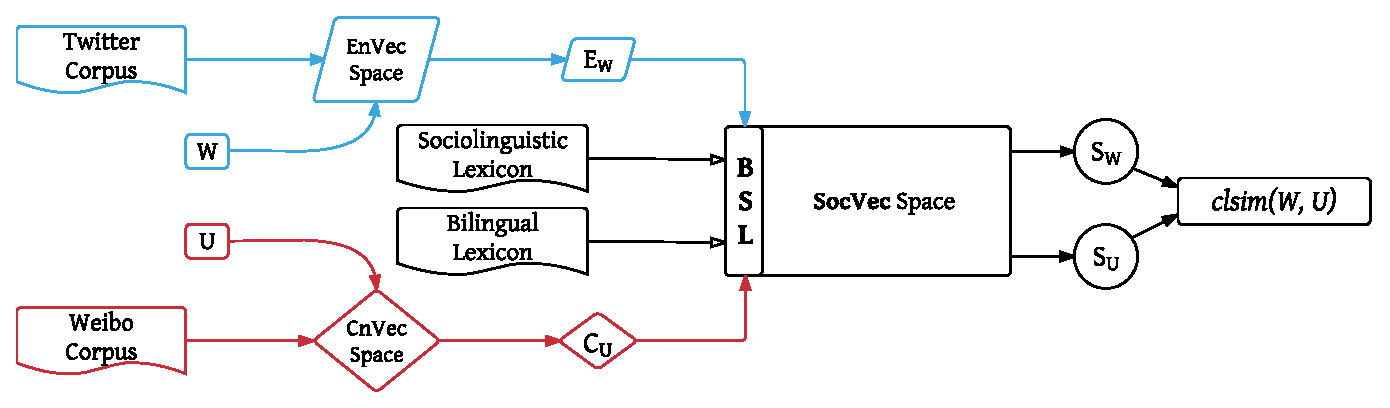
\epsfig{file=figures/overview.pdf, width=0.8\columnwidth}
	\caption{Workflow for computing the cross-cultural similarity between an English word \textit{W} and a Chinese word \textit{U}. $E_x$, $C_x$ and $S_x$ denote the word vectors of word $x$ (either $U$ or $W$) in \textit{EnVec} space, \textit{CnVec} space and \textit{SocVec} space respectively.  }
	\label{fig:overview}
\end{figure}

\subsection{Overall Workflow}
The \textit{\socvec}~model attacks the problem with the help of three low-cost external resources: 
i) English Twitter corpus and Chinese Weibo corpus; ii) a bilingual lexicon (\textit{BL}) between 
 English and Chinese common words;  
iii) English and Chinese socio-linguistic vocabularies 
(\textit{ESV} and \textit{CSV}).
For convenience, the words in these vocabularies are called
{\em social words}. Examples of social words in English include
\textit{fawn, inept, tremendous, gratitude,
terror, terrific, kiss, loving, traumatic}~\footnote{There are open-sourced
resources for these words as Section 3.1.4 describes.}
%\BL{maybe use another expression for the social words} 

\figref{fig:overview} shows the workflow of our framework to construct \textit{\socvec}~and compute $clsim(W,U)$. First, we train English and 
Chinese word embeddings (\textit{EnVec} and \textit{CnVec}) 
on the Twitter and Weibo corpora respectively. Then 
we build a bilingual socio-linguistic lexicon (\textit{BSL}) 
from the bilingual lexicon, CSV and ESV. 
The \textit{BSL} helps us 
map previously incompatible \textit{EnVec} and \textit{CnVec} 
into the common higher-dimensional \textit{\socvec~}space in which
two new vector representations, $S_W$ for $W$ and $S_U$ for $U$,
are now comparable to each other. 

\subsection{SocVec Modeling}
\label{sec:model}
In this section, we present the details of building the \textit{BSL} 
and constructing the \textit{\socvec} space.

\subsubsection{Building the BSL}
The process of building the \textit{BSL} is 
illustrated in~\figref{fig:BSL}. 
We first use the bilingual lexicon to translate each social word 
in the \textit{ESV} into Chinese words and then filter out any Chinese words 
that are not in the \textit{CSV}. After that, we have a set of 
Chinese social words translated from each English social word. 
We call this set of Chinese words the ``translation set''.
The final step is to generate a Chinese ``pseudo-word'' 
for each English social word.\footnote{A pseudo-word can be either 
an existing word that is the most representative word of the translation set 
or a fabricated word whose word vector is the combination of word vectors of
the translation set.}

\begin{figure}[th]
	\centering
	\epsfig{file=figures/BSL.pdf, width=0.9\columnwidth}
	\caption{Generating an entry in BSL for ``\textit{fawn}'' 
		and its pseudo-word ``\textit{fawn}*''.}
	\label{fig:BSL}
\end{figure}

For example, in \figref{fig:BSL}, the
English social word ``\textit{fawn}'' has three Chinese translations in the 
bilingual lexicon, but only two of them are social words. 
The pseudo-word generator takes the word vectors of the two words, namely
奉承(flatter) and 谄媚(toady), as input, and generates the pseudo-word 
vector of ``\textit{fawn}'', denoted as ``\textit{fawn*}''. 
%\footnote{The reason why we use the direction from English to Chinese  is that English socio-linguistic vocabularies tend to be more accessible and accurate than low-resource languages. The filter is optional for low-resource language which has no socio-linguistic lexicon, if we can afford the inaccuracy.}

Given an English social word $s$, we denote $\mathbf{C_i}$ as 
word vector of the $i^{th}$ word of the translation set of
size $N$. We design four types of pseudo-word generator as follows: 

\begin{align*}
	\intertext{\textbf{Max.}: Maximum of the values in each dimension, 
assuming $K$-dimensional word vectors.}
	Pseudo(\mathbf{C_1},...,\mathbf{C_N}) &= \begin{bmatrix}
	max(C_1^{(1)},...,C_N^{(1)}) \\
	\vdots   \\
	max(C_1^{(K)},...,C_N^{(K)})
	\end{bmatrix}^{\rm T} \\
	\intertext{\textbf{Avg.}: Average of the values in each dimension.}
	Pseudo(\mathbf{C_1},...,\mathbf{C_N})&=\frac{1}{N}\sum_i^N\mathbf{C_i} \
	\intertext{\textbf{W.~Avg.}: Weighted average value of each dimension 
with respect to the translation confidence (see~\secref{sec:blpre}).} 
	Pseudo(\mathbf{C_1},...,\mathbf{C_N})&=\frac{1}{N}\sum_i^Nw_i \mathbf{C_i} \
	\intertext{\textbf{Top}: Choose the most confident translation, $\mathbf{C_{top}}$.}
	Pseudo(\mathbf{C_1},...,\mathbf{C_N}) &= \mathbf{C_{top}} \
\end{align*}

At the end of this step, the BSL contains a set of English-Chinese word 
vector pairs, each representing an English social word and 
its Chinese pseudo-word.

\subsubsection{Constructing the \socvec~Space}
\label{sec:pg}
\textbf{Notation Definition.} 
We denote $\bf{E_x}$, $\bf{C_x}$ and $\bf{S_x}$ as the word vectors of 
word $x$ in \textit{EnVec}, \textit{CnVec} and \textit{\socvec} spaces
respectively.  Let $B_i$ be an English word and $B_i^*$ be
the corresponding Chinese pseudo-word in \textit{BSL} of size $L$. 

We can map an English word vector $\bf{E_W}$ into \textit{\socvec} by 
computing the cosine similarity between $\bf{E_W}$ and every English
word vector in \textit{BSL}, effectively constructing a new vector
$\bf{S_W}$ of size $L$. We can similarly map a Chinese word vector 
$\bf{C_U}$ into a new vector $\bf{S_U}$. 
Now $\bf{S_W}$ and $\bf{S_U}$ belong to the same vector space \textit{\socvec} 
and are comparable. 

For example, if $W$ is ``nagoya'' and $U$ is ``名古屋'', we compute the
cosine similarities between ``nagoya'' and ``fawn'', ``inept'', etc. in 
{\em EnVec} space, to form a vector of size $L$. This vector is known
as $\bf{S_{\text{nagoya}}}$. Similarly, we compute the cosine similarities
between ``名古屋'' and the Chinese pseudo-words of 
``fawn'', ``inept'', etc., and form a new vector $\bf{S_{\text{名古屋}}}$. 

Formally, $clsim(W,U)$ is computed as:
{\small
\begin{align*}
&clsim(W,U) := f(\mathbf{E_\text{W}},\mathbf{C_\text U}) \\ 
&=sim\left(
\begin{bmatrix}
    cos(\mathbf{E_\text W},\mathbf{E_{ B_1}})\\
    \vdots \\
    cos(\mathbf{E_\text W},\mathbf{E_{B_L}})
\end{bmatrix}^{\rm T},\begin{bmatrix}
    cos(\mathbf{C_\text U},\mathbf{C_{B_1^*}})\\
    \vdots \\
    cos(\mathbf{C_\text U},\mathbf{C_{B_L^*}})
\end{bmatrix}^{\rm T}\right)\\
&=sim(\mathbf{S_\text W},\mathbf{S_\text U}) 
\end{align*}}
where $cos$ denotes the cosine similarity, 
while $sim$ is a generic similarity function, for which a number of
metrics will be considered later in \secref{sec:eval}.
%
%to project $\mathbf{E_W}$ and $\mathbf{C_U}$ to $\mathbf{S_W}$ and $\mathbf{S_U}$ so that they can be comparable to each other.
%We define the function $f$ to compute cross-lingual similarity between $W$ and $U$ as follows.\footnote{Here $cos$ stands for cosine similarity, } This calculation process is also shown in ~\algref{alg:alg1}. \\
%
%\begin{algorithm}[th]
%	\small
%	\DontPrintSemicolon
%	\caption{Compute cross-lingual similarity between an English word 
%		\textit{W} and a Chinese word \textit{U} } 
%	\label{alg:alg1}
%	\KwIn{ \textit{EnVec}, \textit{CnVec}, $BSL$ with $L$ word pairs} 
%	\KwOut{the cross-lingual similarity $clsim(W,U)$} 
%	$E_W$ = word vector of $W$ in \textit{EnVec}\\
%	$C_U$ = word vector of $U$ in \textit{CnVec}\\
%	$S_W$ =  zero vector with $L$ dimension \\
%	$S_U$ =  zero vector with $L$ dimension \\
%	%	\Comment*[l]{Project $E_W$ into $S_W$}
%	\For{$1 \le i \le L$}{
%		$B_i$ =  $i^{th}$ English word in \textit{BSL} \\
%		$B_i^*$ = Chinese pseudo-word of $B_i$ \\
%		$S_W[i]$ = $cos(E_W,E_{B_i})$\\
%		$S_U[i]$ = $cos(C_U,C_{B_i^*})$\\
%	} 
%	\Return $clsim(W,U)$ = $sim(S_W,S_U)$\\
%\end{algorithm}
%\begin{figure}[th!]
%	\centering
%	\epsfig{file=figures/SocVec.pdf, width=0.6\columnwidth}
%	\caption{Using \textit{BSL} to project $E_W$ and $C_U$ to $S_W$ and $S_U$.}
%	\label{fig:swsu}
%\end{figure}

%\subsubsection{Parameters Description}
%\label{sec:pd}
%Here, we briefly summarize the main parameters of \textit{SocVec} model:
%\begin{itemize}
%\item Two trained monolingual word embeddings, \textit{EnVec} and \textit{CnVec};  
%\item A bilingual lexicon;
%\item Chinese and English socio-linguistic vocabularies; 
%\item Pseudo-word generator function; 
%\item Option of similarity function $sim$; 
%\end{itemize} 
%We conduct several experiments for testing the these parameters in~\secref{sec:mcdne}.

%	\section{Experiment}
In this section, we experiment on different NLG tasks. We first present the experimental setup on different tasks. Then, we show the quantitative and qualitative results together with comprehensive analysis and ablation studies.

\subsection{Implementation Details}
We evaluate the newly proposed ICL strategy on five commonly-researched natural language generation tasks: reading comprehension, dialogue summarization, style transfer, question generation and news summarization. Details on the task description, the strong baseline, corresponding  dataset, evaluation metrics and key hyper-parameters for each task are presented as follows.

\begin{table*}[th]
	\scriptsize
	\centering
	\begin{tabular}{lp{1.1cm}rrrcccc}
		\hline
		Task & Dataset & \#Train & \#Val & \#Test & Input & Output & Avg & Std\\
		\hline
		Reading Comprehension & DREAM & 6,116 & 2,040 & 2,041 & ``Q:''+ question + dialogue & answer & 5.59 & 2.61\\
		Dialogue Summarization & SAMSum & 14,732 & 818 & 819 & dialogue & summary  & 24.99 & 13.06\\
		Style Transfer & Shakespeare & 36,790 & 2,436 & 2,924 & original/modern  & modern/original  & 11.63 & 8.19 \\
		Question Generation & SQuAD1.1 & 75,722 & 10,570 & 11,877 & passage + [SEP] + answer & question & 13.09 & 4.27 \\
		News Summarization & CNNDM & 287,227& 13,368& 11,490 & document & summary & 70.97 & 29.59\\ 
		\hline
	\end{tabular}
	\caption{A summary of tasks and datasets. \#Train, \#Val and \#Test refers to the number of samples in the corresponding dataset. Avg and Std are the statistics for the number of output tokens. ``+'' refers to the concatenation operation.}
	\label{tab:taskdata}
\end{table*}

\textbf{Reading comprehension} is the task that answering questions about a piece of text. We use the DREAM dataset~\cite{sun2019dream} where questions are about corresponding dialogues and the answer is a complete sentence in natural language. We neglect the negative choices in the original dataset and formulate it as a NLG task. We adopt the pre-trained language model BART~\cite{lewis2020bart} as the baseline, where the input is a concatenation of a question and the corresponding dialogue made up of speakers and utterances. 
We experiment with  transformers\footnote{\url{https://github.com/huggingface/transformers}} based on the publically available ``facebook/bart-large'' checkpoint \footnote{\url{https://huggingface.co/facebook/bart-large}}.
%The preceding BART model is also adopted as the baseline, whereas the input is a concatenation of question and a dialogue.
The generated answers are evaluated by BLEU scores\footnote{The BLEU-1/2/3/4 scores are computed according the Google's implementation(\url{https://github.com/tensorflow/nmt/blob/master/nmt/scripts/bleu.py}).}~\cite{papineni2002bleu} widely used for QA systems, together with Meteor and Rouge-L F1 as mentioned above. The parameters are also the same as dialogue summarization, except that the early-stop is activated if there is no improvement on the perplexity of the validation set. 


\textbf{Dialogue summarization} is to generate a concise summary covering the salient information in the input dialogue. The preceding model BART has shown to be a strong baseline for this task, where only the dialogue is concatenated into a single sequence as the input. We experiment with  %transformers\footnote{\url{https://github.com/huggingface/transformers}} based on the publically available ``facebook/bart-large'' checkpoint \footnote{\url{https://huggingface.co/facebook/bart-large}} and 
SAMSum dataset\footnote{\url{https://arxiv.org/src/1911.12237v2/anc/corpus.7z}}~\cite{gliwa2019samsum} for daily-chat dialogues. 
The generated summaries are evaluated by comparing with the reference through evaluation metrics, including Rouge-1/2/L F1 scores\footnote{\url{https://github.com/pltrdy/files2rouge}}~\cite{lin2004rouge}, Meteor~\cite{banerjee2005meteor} and BertScore F1\footnote{Both Meteor and BertScore are calculated by SummEval(\url{https://github.com/Yale-LILY/SummEval}), and the latter one is based on the default bert-base-uncased model.}. We evaluate the model on the validation set after each training epoch and the early-stop patience will be added 1 if there is no improvement according to the Rouge-2 F1 score. The training process terminates when the early-stop patience equals or is larger than 3.  During the inference, the minimum and maximum output length is set to 5 and 100 respectively, with no\_repeat\_ngram\_size=3, length\_penalty=1.0 and num\_beams=4.


% The answer is either a span of words in the original text or a complete sentence in natural language.
\textbf{Style transfer} preserves the semantic meaning of a given sentence while modifies it's style, such as positive to negative, formal to informal, etc.
We adopt the Shakespeare author imitation dataset~\cite{xu2012paraphrasing}, containing William Shakespeare's original plays and corresponding modernized versions. Krishna el al.~\shortcite{krishna2020reformulating} proposed to do unsupervised style transfer by training paraphrase models based on the GPT-2 language model~\cite{radford2019language}. We re-implemented their approach STRAT\footnote{\url{https://github.com/martiansideofthemoon/style-transfer-paraphrase}} and evaluated with the provided script. Evaluation metrics includes 
transfer accuracy(ACC), semantic similarity(SIM), Fluency(FL) and two aggregation metrics, i.e., geometric averaging(GM) and their newly introduced $J(\cdot)$ metric. The hyper-parameter $hp$ equaling 0.0, 0.6 or 0.9  in Table~\ref{tab:end2endst} is the sampling parameter for trades off between ACC and SIM in their approach. 
In the training stage, we evaluate the model after updating every 500 steps. The perplexity on the validation set is used to activate the early-stop which equals 3. The inference is done as default.
 
\textbf{Question generation}~\cite{zhou2017neural} aims at generating a question given an input document and its corresponding answer span. SQuAD 1.1~\cite{rajpurkar2016squad} is generally used for evaluation. We adopt the data split as in \cite{du2017learning} and fine-tune the pre-trained UniLM~\cite{dong2019unified} as the strong baseline according to their official implementation\footnote{\url{https://github.com/microsoft/unilm/tree/master/unilm-v1}}. Generated questions are evaluated by metrics including BLEU-1/2/3/4, Meteor and Rouge-L with the provided scripts. The model is evaluated every 1000 steps and the early-stop equaling 3 is associated with the perplexity on the validation set. Other parameters are unchanged following the official guideline.

\textbf{News summarization} differs from dialogue summarization where the input is a document instead of a dialogue. We adopt the same strong baseline BART and evaluation metrics as dialogue summarization. Experiments are done with CNNDM dataset~\cite{HermannKGEKSB15} consisting of news articles and multi-sentence summaries\footnote{\url{https://github.com/pytorch/fairseq/blob/main/examples/bart/README.summarization.md}}. The model is evaluated every 2000 steps and the early-stop equaling 3 is associated with the Rouge-2 on the validation set. During the inference, the minimum and maximum output length is set to 45 and 140 respectively, with no\_repeat\_ngram\_size=3, length\_penalty=2.0 and num\_beams=4.
%\footnote{Inference parameters are borrowed from \url{https://github.com/pytorch/fairseq/blob/main/examples/bart/summarize.py}}

The summary of each task is listed in Table~\ref{tab:taskdata}. For fair comparisons, we re-implemented baselines following the above instructions on our machine. On top of the above baselines, we further arm them with the ICL strategy according to the Algorithm~\ref{alg:picl}. The settings of newly introduce Start and Stride are specified and discussed in following sub-sections. All of our experiments are done on a single RTX 3090 or a single RTX 2080Ti with 24G and 11G GPU memory respectively.
%and the result are averaged over three runs.


 
\subsection{Automatic Evaluations on Different Tasks}
\label{sec:taskperformances}

We compare our approach with the vanilla models mentioned above and the approach from~\citet{liang-etal-2021-token-wise} as baselines.
The performances on different NLG tasks are shown in Table~\ref{tab:end2end}. 
These tasks not only focus on solving different problems, but also has various amount of training data as well
as reference output lengths as shown
Table~\ref{tab:taskdata}.
Besides, the basic model are also different, including BART, GPT-2 and UniLM. 
Our new training strategy achieves significantly improvements among different tasks on most evaluation metrics, which shows that our method not only works well, but also has strong generalization abilities.

We explain the some specific results as follows:

(1) Our training strategy boosts the performances of the original STRAT with different $hp$ in the style transfer task. GM and J are two comprehensive evaluation metrics, with our approach topping the ranks with significant improvements.

(2) TCL generally performs poorly on tasks
with more training data. For example, it failed on question generation without any improvements over the vanilla model under the same parameter setting, while ICL still 
logs gains. This is mainly due to two reasons.
First, because the nature of TCL is data augmentation which is more effective in low-resource settings,
when training data is abundant, it becomes less useful. 
Second, the way they calculate the loss as sub-sequence generation better suites paraphrasing tasks, such as machine translation tested in their paper, as the order of 
the corresponding tokens between input and output 
are almost the same. Learning such forward mapping can 
be regarded as a kind of ``easy-to-hard'' 
in these limited scenarios.
However, this doesn't hold true for other tasks, 
such as summarization and question generation. 
Therefore, we didn't further test it on CNNDM since
CNNDM has the large amount of training data among
the five.

(3) For news summarization, Rouge-1 scores (precision, recall) for the baseline and our method on CNNDM are (38.16, 52.72) and (40.84, 49.23) correspondingly. Our method made substantial improvements on the precision with a compromise on the recall. 
The meteor score based on the unigram precision and recall emphasizes more on the recall than the Rouge-1 F1. As a result, it drops while Rouge-1 F1 increases. Overall, our method still outperforms BART on this task, especially on F1 scores of Rouge-2 and Rouge-L.




\begin{table}[th]
	\small
	\centering
	\begin{subtable}{\linewidth}
		\scriptsize
		\centering
		\begin{tabular}{lcccccc}
			\hline
			{Method} & {B1} & {B2} & {B3} & {B4} & {Met} & {RL}\\
			\hline
			w/o CL &  32.03 & 16.01 & 8.77 & \textbf{4.80} & 19.84 & 38.89\\
			TCL & 32.53 & 16.25 & 8.52 &4.67 &19.88 & 39.65 \\
			ICL &  \underline{\textbf{33.99}} & \underline{\textbf{17.43}} & \underline{\textbf{9.18 }}& 4.64 & \textbf{20.60} & \textbf{40.78}\\

			\hline
		\end{tabular}
		\caption{Reading Comprehension}
		\label{tab:end2endrc}
	\end{subtable}
	\\[5pt]
	\begin{subtable}{\linewidth}
		\scriptsize
		\centering
		\begin{tabular}{lccccc}
			\hline
			{Method} & {R1} & {R2} & {RL} & {Met} & {BertS} \\
			\hline
			%BART & 52.60&27.00 &42.10 &- & - \\
			w/o CL & 51.88 & 27.30 & 42.77 & 24.75 & 71.38 \\
			TCL  & 52.33 & 27.80 & \textbf{43.91} & 24.59 & 71.77 \\
			ICL & \underline{\textbf{53.07}} & \underline{\textbf{28.23}} & {43.83} & \underline{\textbf{26.12}}& \underline{\textbf{72.17}} \\
			
			\hline
		\end{tabular}
		\caption{Dialogue Summarization}
		\label{tab:end2endds}
	\end{subtable}
	\\[5pt]
	\begin{subtable}{\linewidth}
		\scriptsize
		\centering
		\begin{tabular}{lcccccc}
			
			\hline
			{Method}&$hp$ &  {ACC} & {SIM} & {FL} & {GM} & {J}\\
			\hline
			%\multirow{3}{*}{STRAT}& 0.0 & 71.70 & \textbf{56.40} & 85.20 & 70.10 & 34.70 \\
			%& 0.6 & 75.70 & 53.70 & 82.70 & 69.50 & 33.50 \\
			%& 0.9 & 79.80 & 47.60 & 71.70 & 64.80 & 27.50 \\
			%\hline
			\multirow{3}{*}{w/o CL}& 0.0 & 70.49 & 55.70 & 85.98 & 69.63& 33.72 \\
			& 0.6 &75.31 & 53.46 & 82.56 & 69.27& 33.30\\
			& 0.9 & 78.76 & 47.38 & 74.42 &65.24 & 27.88\\
						\hline
			\multirow{3}{*}{TCL } & 0.0 & 70.31 & \textbf{55.95} &\textbf{87.24} &  70.01& 34.71 \\
			& 0.6 & 74.79 & 53.14 & 82.56 & 68.97 & 33.21 \\
			& 0.9 & 79.41 & 46.88 & 71.92 &64.45 & 26.92 \\
			\hline
			\multirow{3}{*}{ICL}& 0.0 & \underline{73.72} & 55.91 & 86.30 & \underline{\textbf{70.60}} &\underline{\textbf{35.81}}\\
			& 0.6 & 77.26 & \underline{53.80} & \underline{83.87} & \underline{70.38} & 34.64\\
			& 0.9 & \textbf{79.65} & 48.16 & 76.06 & 66.32 & 29.03\\

			\hline
		\end{tabular}
		\caption{Style Transfer.}
		\label{tab:end2endst}
	\end{subtable}
	\\[5pt]
	\begin{subtable}{\linewidth}
		\scriptsize
		\centering
		\begin{tabular}{lcccccc}
			\hline
			{Method} & {B1} & {B2} & {B3} & {B4} & {Met} & {RL}\\
			\hline
			w/o CL & \textbf{50.38} & 35.67 & 27.24 & 21.36 & 24.40 & 50.67 \\
			TCL &\textbf{50.38} & 35.67 & 27.24 & 21.36 & 24.40 & 50.67\\
			ICL &  50.18 & \textbf{35.72} & \textbf{27.36} & \textbf{21.54} & \textbf{24.57} & \underline{\textbf{51.09}} \\
			\hline
		\end{tabular}
		\caption{Question Generation}
		\label{tab:end2endqg}
	\end{subtable}
		\\[5pt]
	\begin{subtable}{\linewidth}
		\scriptsize
		\centering
		\begin{tabular}{lccccc}
			\hline
			{Method} & {R1} & {R2} & {RL} & {Met} & {BertS}\\
			\hline
			%BART &  \\
			w/o CL &  43.07 & 20.01 & 35.94 & \textbf{21.44} & 63.72 \\
			TCL & - & -&- &- &- \\
			ICL & \textbf{43.39} & \underline{\textbf{20.55}} & \underline{\textbf{36.63}} & 19.68 & \textbf{64.05}\\
			\hline
		\end{tabular}
		\caption{News Summarization}
		\label{tab:end2endns}
	\end{subtable}
	\caption{Performances on different NLG tasks. ICL represents the models trained with our ICL algorithm. TCL refers to the previous work from~\cite{liang-etal-2021-token-wise}. Scores underlined are statistically significantly better than both re-implemented baselines with $p<0.05$ according to t-test. }	
	\label{tab:end2end}
\end{table}


\subsection{Human Evaluations}

To further prove the improvement of ICL, we hired three proficient English speakers for human evaluation. 20 samples from the test set of each task are randomly selected, ignoring the ones with totally same generations among three models, including the vanilla model, TCL and ICL. The original input, reference output and three generations are shown to annotators together, while the order of three generations are unknown and different among samples. 3-point Likert Scale is adopted for scoring for each generation~\cite{gliwa2019samsum}, where [1, 3, 5] represent 
excellent, moderate and disappointing results 
respectively. The average scores and agreements 
among the annotators are shown in 
Table~\ref{tab:humaneval}.

The Fleiss Kappa on the first four tasks indicates the fair to moderate agreements. It shows the promising improvement of ICL over the vanilla model and TCL especially on DREAM, SAMSum, and SQuAD1.1, which is consistent with the conclusion based on automatic metrics.
Although the agreement on style transfer is fair, 
our annotators without Shakespeare background 
tend to give low scores to all outputs.
Therefore, the absolute improvement is 
only $0.04$ compared to both baselines.
%This mainly due to the indistinguishable styles between
%Shakespeare’s plays with are quite different from modern languages. 
Besides, the poor agreement on CNNDM reflects the 
diverse concerns of summarization from different 
annotators. Without more specific instructions, they 
tends to focus more on the content coverage instead 
of checking the detailed facts. This is also 
consistent with the higher Meteor scores of the 
vanilla model over ICL.

\begin{table}[th]
	\scriptsize
	\centering
	\begin{tabular}{l|ccc|c}
		\hline
		{Datasets} & {w/o CL} & {TCL} & {ICL} & {Agreement}  \\
		\hline
		DREAM  &3.07 & 2.50&3.20 &0.48 \\
		SAMSum &2.97 &3.57 &3.97 &0.40 \\
		Shakespeare &2.23 &2.23 & 2.27&0.32 \\
		SQuAD1.1 &3.43 & 3.43 &3.77 &0.35 \\
		CNNDM & 3.45 &- &3.40 &0.11 \\
	%	\hline
	%	overall & & & &\\
		\hline
	\end{tabular}
	\caption{Human evaluations. The agreement is calculated by Fleiss Kappa.}
	\label{tab:humaneval}
\end{table}




%Following Liu et al.\shortcite{liu2021competence}'s work, we asked annotators to comparing the performance between our generated results and baselines by choosing from ``Better, Tie, Worse''. 
%The counts for each choice are shown in Table~\cite{}, where the Fleiss Kappa among annotators is ??.

%Analysis





%\subsection{Analysis on Variable Generation Lengths}

%Teacher forcing, which predicts each token given the reference summary tokens during training and given the previous generated tokens during inference, leads to the exposure bias problem for NLG tasks.
%Since ICL starts the training process by predicting the last few tokens of outputs and gradually calculates the loss based on more tokens when the model is stronger, we hypothesis that it can alleviate the exposure bias for training Seq2Seq models to some extent.
%As stated in~\cite{pang2020text}, the output quality tends to degrade as the output length increase with the exposure bias.
%So, we divided the test set of each task according to the length of the generated output into 4 buckets and randomly picked 20 samples in each buckets for both the corresponding baselines and our approach. Each generation is annotated by 5 point Likert Scale, where 1 is the worst and 5 is the best. 

%The trends of performances on variable generation lengths are in Figure~\ref{}.


%	\section{Related Work}
This section surveys previous works on question generation and tree encoding
respectively.

Text question generation has attracted the attention 
after the work of ~\citeauthor{du2017learning}~\shortcite{du2017learning}, who uses deep seq2seq model 
to generate questions from a raw text paragraph. 
Before that, text question generation relied heavily on hand-craft 
question patterns~\cite{HeilmanS10,LabutovBV15,MostowC09} which is time and 
labor consuming. 

However, this pure seq2seq model is not focused and 
has no control over part in the paragraph to generate question. 
~\citeauthor{zhou2017neural}~\shortcite{zhou2017neural} proposed to encode 
key phrase information using binary indicators to generate 
key-aware questions and they assumes the answer to be key phrase. 
Considering key phrase (answer) is unavailable in reality, 
~\citeauthor{SubramanianWYT17}~\shortcite{SubramanianWYT17} applied 
a two-stage approach. First, key phrases are extracted by 
pointer network~\cite{ptrnet}. Second, 
key phrases are encoded in the same way as 
Zhou et al. With the intuition that questions could be asked in many ways, 
~\citeauthor{Yao2018vae}~\shortcite{Yao2018vae} used conditional-VAE to 
increase the diversity of questions. More recently, models with 
auxiliary feature information~\cite{HarrisonW18} helped improve 
the question quality. Structure question generation aims at 
converting structured data such as triples in knowledge graph to questions. 
~\citeauthor{SerbanGGACCB16}~\shortcite{SerbanGGACCB16} proposed a model to generate factoid questions from knowledge base triples.  None of the above work
considered using parse tree structures to aid question generation process,
which is the focus of this paper.

Sequential RNN model takes sentence as a sequence of words, 
ignoring the syntactic information. In order to utilize
such syntactic information with sequential information, 
~\citeauthor{tai2015improved}~\shortcite{tai2015improved} proposed Tree-LSTM to 
encode the binary parse tree recursively in a bottom-up fashion to 
classify sentiment. In text generation task, 
\citeauthor{eriguchi2016tree}~\shortcite{eriguchi2016tree} 
proposed a tree-to-sequence model with attention mechanism to do 
machine translation and 
~\citeauthor{liang2018automatic}~\shortcite{liang2018automatic} proposed a 
tree-to-sequence model which could handle arbitrary trees, 
to do code comment generation. Our work is inspired by these previous
attempts and we are first to adapt structure encoded neural models to
textual question generations.
%	\section{Conclusion}
\label{sec:conclude}
In this work,
we propose a new data creation method to generate
 a semi-structured synthetic training data for 
opinion summarization,
which is known for lacking training data.
\cut{We showed that by extracting an aspect-opinion pairs and 
implicit sentences from multiple reviews
first and then synthesizing them into semi-structured data, we achieve
better performance on opinion summarization.}
%\KZ{It is critical to show in your experiments that the proposed
%synthetic data is better than other possible alternatives.}, 
We also designed an aspect-guided model with opinion-aspect pair encoder and implicit sentence encoder.
The results showed that
the proposed model can make full use of semi-structured data
and generate high-quality summaries.



 
	\bibliographystyle{aaai}
	\bibliography{aaai}
	
\end{CJK}

\end{document}
